\documentclass[12pt]{article}

\usepackage{scicite,times,graphicx,float,hyperref}
\usepackage[skip=0pt]{caption}
\usepackage[utf8]{inputenc}
\usepackage{enumitem}
\usepackage{booktabs}
\usepackage{multicol}

\topmargin -1.0cm
\oddsidemargin 0.0cm
\textwidth 16cm 
\textheight 23cm
\footskip 1.0cm

\newenvironment{sciabstract}{%
\begin{quote} \bf}
{\end{quote}}

\newcounter{lastnote}
\newenvironment{scilastnote}{%
  \setcounter{lastnote}{\value{enumiv}}%
  \addtocounter{lastnote}{+1}%
  \begin{list}%
  {\arabic{lastnote}.}
  {\setlength{\leftmargin}{.22in}}
  {\setlength{\labelsep}{.5em}}
}
{\end{list}}

\title{Simulation of a Scientific Computation Platform\\With a Focus on Quality Attributes} 

\author
{Filipe Pires [85122], João Alegria [85048]\\
\\
Software Architecture\\
\normalsize{Department of Electronics, Telecommunications and Informatics}\\
\normalsize{University of Aveiro}\\
} 

\date{\today{}}

%%%%%%%%%%%%%%%%% END OF PREAMBLE %%%%%%%%%%%%%%%%%%%%%

\begin{document}

\baselineskip18pt

\maketitle

\section*{Introduction} %%%%%%%%%%%%%%%%%%%%%%%%%%%%%%%%%%%%%%%%%%%%%%%%%%%%%%%%%%%%%%%%%%%%%%%%%%%%%%%%%%%%%%%%%%%%%%%%%%%%%%%%%%%%%%%%%%%%%%%%%%%%%%%%%%%%%%%%

This report aims to describe the work developed for the third and final assignment of the course of 'Software Architecture', focused on a platform that accepts
and processes computational services requested by the scientific community.

The aim of the assignment was to design and develop a software architecture relying on four of the most relevant quality attributes:
performance, availability, scalability and usability.
Playing the role of software architects, we came up with the solution for an infrastructure for our stakeholder.
The platform here presented is capable of deploying a cluster of servers monitored by a tactic entity and whose requests from clients are distributed by a load balancer.
Although the cluster is locally simulated, the configuration is done so that it is possible to deploy in a distributed environment.

So in this report we present the architecture of our solution, justifying design decisions according to what we learned and found to be most suitable for our use case.
We also mention how the work was distributed amongst the authors.

All code developed is publicly accessible in our GitHub repository:

\url{https://github.com/FilipePires98/AS/}

% \vspace{-10pt}
% \begin{itemize}[noitemsep]
%   \item Prepare - the selected farmers move to a Standing Area, ready for orders.
%   \item Start - the actual simulation begins and farmers start moving.
%   \item Collect - farmers collect corn cobs from the Granary (where the cobs initially are).
%   \item Return - farmers return to the Storehouse with the collected corn cobs.
%   \item Stop - farmers stop whatever they are doing and return to the Storehouse.
%   \item Exit - simulation ends and the program closes.
% \end{itemize}
% \vspace{-10pt}

% \begin{figure}[H]
%   \centering
%   \begin{minipage}{\textwidth}
%     \centering
%     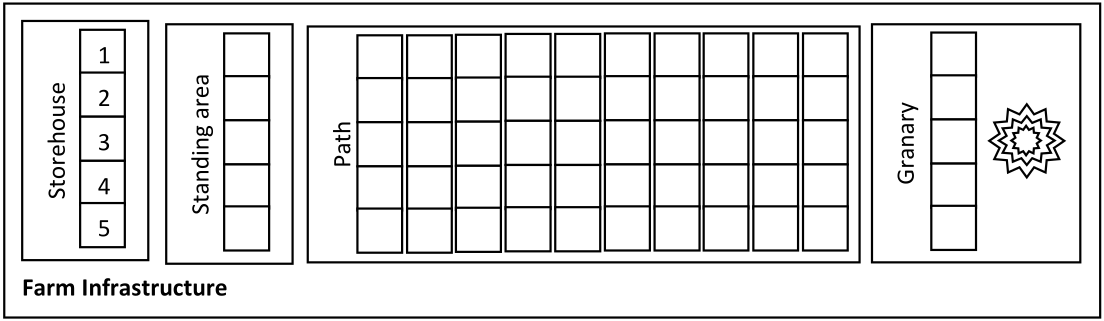
\includegraphics[width=\linewidth]{img/Design_FI.png}
%   \end{minipage}%
%   \caption{Visual representation of the farm, taken from \cite{assign}.}
%   \label{Design_FI}
% \end{figure} 

%\texttt{java -cp <userdir>/build/classes fi.FarmInfrastructure}

\newpage
\section{Scientific Computation and Custom Systems} \label{scientificcomputation} %%%%%%%%%%%%%%%%%%%%%%%%%%%%%%%%%%%%%%%%%%%%%%%%%%%%%%%%%%%%%%%%%%%%%%%%%%%%%%

Applied computer science and mathematics often use advanced computing capabilities to understand and solve complex problems.
In practical use, computational science is typically the application of computer simulation and other forms of computation to tackle problems in various
scientific disciplines.
Scientists and engineers develop computer programs that model systems being studied and run these programs with various sets of input parameters.
In some cases, these models require massive amounts of calculations and are often executed on supercomputers or distributed computing platforms.

This project does not describe one of these models, rather it is about the development of an infrastructure capable of supporting such computationally demanding tasks.
The adopted strategy was of coordinating a cluster of processing servers.
The following tactics were selected to be implemented:
\vspace{-10pt}
\begin{itemize}[noitemsep]
  \item Computation Replicas - requests must be fairly distributed amongst the servers.
  \item Concurrency - each request runs on its own thread in a server.
  \item Redundancy - in case a server goes down, requests should be reallocated.
  \item Monitor - everything must be supervised, from the cluster's status, to the clients' identification and request treatment.
  \item Horizontal scalability - new servers can be deployed whenever necessary.
\end{itemize}
\vspace{-10pt}

\subsection{The Scenario} \label{scenario} %%%%%%%%%%%%%%%%%%%%%%

In order to test the application of the infrastructure on a scientific problem, an example scenario was adopted: the calculation of the mathematical constant $\pi$ (pi).
Being an irrational number, $\pi$ cannot be expressed as a common fraction and its decimal representation never ends and never settles into a permanently repeating pattern.
Nevertheless, in the 21st century, mathematicians and computer scientists have pursued new approaches that, when combined with increasing computational power,
extended the decimal representation of $\pi$ to many trillions of digits \cite{pisky}.
The primary motivation for these computations is as a test case to develop efficient algorithms to calculate numeric series, as well as the quest to break records.

The most commonly adopted forms of calculating $\pi$ are the iterative algorithms \cite{jorg}.
In order to only focus on the infrastructure's implementation, while simulating the actual implementation of the iterative algorithms, a control variable
corresponding to the number of iterations to be used on the calculation was introduced to regulate servers' response times.

\subsection{The Messages} \label{messages} %%%%%%%%%%%%%%%%%%%%%%

One of the fundamental constraints applied to our implementation was related to communications.
Each individual server is launched as an independent process.
This is also true for each individual client.
The orchestrator runs in an independent process as well, serving as both a load balancer and a tactic monitor - although these two are built as separate entities.
So in order for entities to communicate with each other, the TCP/IP socket technology was made a requirement.

For simplicity, only two service message types were defined:
\vspace{-10pt}
\begin{itemize}[noitemsep]
  \item Request: $|$ \texttt{clientID} $|$ \texttt{requestID} $|$ \texttt{01} $|$ \texttt{\# iterations} $|$
  \item Reply: $|$ \texttt{serverID} $|$ \texttt{clientID} $|$ \texttt{requestID} $|$ \texttt{02} $|$ \texttt{\# iterations} $|$ \texttt{pi} $|$
\end{itemize}
\vspace{-10pt}
In them are the following parameters:
\texttt{clientID}, a positive integer that uniquely identifies a client machine;
\texttt{serverID}, a positive integer that uniquely identifies each physical server in the cluster;
\texttt{requestID}, a positive integer that uniquely identifies a pi calculation request (computed as 1000 $\times$ \texttt{client id} $+$ increment);
\texttt{01} and \texttt{02}, the request and reply codes;
\texttt{\# iterations}, the chosen value for the previously mentioned control variable used to simulate the number of iterations for the computation of pi
(each iteration / cycle corresponds to 1 second);
\texttt{pi}, the computed value of $\pi$.

A few additional message types were added during development for management purposes:
\vspace{-10pt}
\begin{itemize}[noitemsep]
  \item Heartbeat: ..................................
\end{itemize}
\vspace{-10pt}

..............................................................................................

\newpage
\section{System Architecture} \label{architecture} %%%%%%%%%%%%%%%%%%%%%%%%%%%%%%%%%%%%%%%%%%%%%%%%%%%%%%%%%%%%%%%%%%%%%%%%%%%%%%%%%%%%%%%%%%%%%%%%%%%%%%%%%%%%%

The adopted architecture was a hybrid version of client/server and master/slave.
First of all, the clients that connect to and use our system act as a typical client entity and, from their perspective, there is only one server entity 
responding to their requests.
The server, however, is in fact made up of several entities, each with its specific responsibility.
These internal entities are independent from one another and when they need to communicate they do so in a client/server manner, making the necessary requests 
and awaiting for a response.

The architecture follows a master/slave model as well in the sense that the $\pi$ calculation infrastructure is comprised of a main entity (the master) and a 
set of calculation servers (the slaves): the calculation servers await for their master to assign them tasks; the main entity is actually made up of two 
entities (a Load Balancer and a Tactic Manager) that run in the same process as we will detail further ahead and that does the interaction with the clients and 
communicate with the slaves in order to deliver a response to the client requests.

As predefined by our stakeholder, all communications are done through web sockets.
Below, we provide a detailed description of each entity as well as of the communication mechanisms.

\subsection{Entities} \label{entities} %%%%%%%%%%%%%%%%%%%%%%%%%%

\subsubsection{Client}

The Client acts as the system entity that provides the user a graphical interface (GUI) in order to make calculation requests to the scientific computation 
platform.
It is the Client that parses the user input and sends requests to the Load Balancer, awaiting for responses to arrive to provide the user with the answers he/she needs.
The user can make how many requests he/she desires, as the Client does not need to wait for each computation response in order to request another.

A key design decision was made when implementing the communication mechanism for clients.
After some deliberation, we concluded that the best approach for the web sockets' ports definition would be to make the Client responsible for choosing the port
it uses, since there could be constraints related to the machine where the process is running and it wouldn't be viable for the Client to receive the port 
indication from a server that might have no knowledge about the ports already in use on the Client's machine. 
This way, the Client instantiates a web socket with a port defined by itself, allowing the computation responses to be sent to it asynchronously.

A Client instantiation imposes the exchange of some control messages.
When initiating, the Client needs to send a message to notify the main server that it was created, indicating its web socket host IP address and chosen port.
In response, the main server sends to the Client an internal identifier (used for the server to recognize it in future messages).
When the Client is stopped, it sends a new message notifying the main server that it will shut down. 

\subsubsection{Calculation Server}

Calculation servers hold the code for the computation of the scientific algorithms.
These entities await for requests to arrive from the main server, process them and respond directly to the clients that triggered the requests.
For our use case, the $\pi$ computation algorithm is simulated according to a parameter, as previously mentioned.
Nevertheless, the code was made so that a real algorithm implementation can quickly replace the current simulation, and allowing additional algorithms to be 
inserted so that the platform supports new computation requests.

A Server is able to respond directly to the Client thanks to an internal mechanism:
the request is initially sent by the Client to the Load Balancer;
the Tactic Manager then adds the Client metadata to it and the Load Balancer forwards the updated message to the Calculation Server;
with the added information, the Server gains the capacity to send the computation results to the Client without the help of the main server.
All processing of requests is parallelized, preventing any undesired bottlenecks.

Similarly to the Client, a Server needs a web socket server to receive the calculation requests, so it also needs to choose the port it will be active in. 
The same physical constraints apply, so the servers need to exchange similar control messages on instantiation and shut down, including host IP address and port identification.

\subsubsection{Load Balancer} \label{lb}

We have mentioned the Load Balancer more than once, as it is a key asset to our solution, and in this section we explain why it is one of the most important 
entities of our architecture.
Its existence started by being a project requirement, but we quickly understood its actual importance when handling the quality attributes we wished to guarantee.

Load Balancer's main purpose, as the name implies, is to distribute in a balanced way the incoming $\pi$ calculation requests across all registered servers. 
When one or more calculation requests are sent to it, Load Balancer asks the Tactic Manager via web socket to identify the least occupied Server and assigns the 
task to that Server.
It is in this stage, after the Server is chosen, that the Load Balancer asks the Tactic Manager for the Client's metadata to be inserted in the request.

It is important to state that the Load Balancer is the central entity of the infrastructure.
It is only through it that the clients are able to interact with the remainder of the infrastructure and it is only this entity that the Client has knowledge 
about from the very moment it is instantiated.
The Tactic Manager only server this entity, although it holds the information about the remainder.
If the process where the Load Balancer and Tactic Manager are running dies for some reason, the platform will not work; this is not true for the Client nor the 
Calculation Server.
In section \ref{constraints} we explore how the Load Balancer is able to handle availability and scalability.

\subsubsection{Tactic Manager}

If the Load Balancer is the heart of the platform, the Tactic Manager can easily be considered its brain.
It is this entity that holds the knowledge about every registered Server, every connected Client, the state of each and all, and who is processing each request 
at any time.
With this knowledge, it is able to understand which Server has the least amount of pending requests (is least occupied) and provide the Load Balancer with an 
informed answer.
The shared GUI of the Load Balancer and Tactic Manager is always up-to-date because of this knowledge as well.

Although the Calculation servers receive messages from the Load Balancer, they only communicate with the central server through the Tactic Manager (they only 
send messages to it). 
The Server initialization and shutdown control messages are sent to the Tactic Manager, that will process and store the information, also sending back the 
created identifier in case of the Server creation.
Additionally, all servers when receiving or finishing the processing of a calculation request should notify this management entity of their status change.

A control mechanism already mentioned in section \ref{messages} but not yet explained is also responsibility of the Tactic Manager - the health-check of 
registered servers.
This feature was added as we concluded it would be paramount when assuring some quality attributes, namely availability, performance and usability.
The flow of this process goes as follows: when the Tactic Manager is created, the Health-checking subprocess is initiated in parallel; from then on, this
subprocess sends health checks to all registered servers on a time interval established \textit{a priori} (in our scenario it was defined as 30 seconds periods);
in the event that one Server does not respond, it is considered dead and consequently deleted from the internal registries so that future requests are not sent 
to it; if any requests assigned to the dead Server were incomplete, these are sent back to the Load Balancer for redistribution amongst the living Servers.

\subsection{System Components} %%%%%%%%%%%%%%%%%%%%%%%%%%%%%%%%%%

We have discussed the entities that make up the logic of the solution - these are all represented in our architecture diagram in Figure \ref{pa3Arch}.
However, there are additional system components that provide what is necessary for the integration of the whole infrastructure, some of them worth exploring in 
depth due to their important roles.

The first two important components are the LoadDistributer, a class internal to the LoadBalancer that is responsible for the actual distribution of incoming requests, 
and the HealthChecker, internal to the TacticManager with the duty to health check all registered servers and take action in case any of them does not respond.

\begin{figure}[H]
  \centering
  \begin{minipage}{\textwidth}
    \centering
    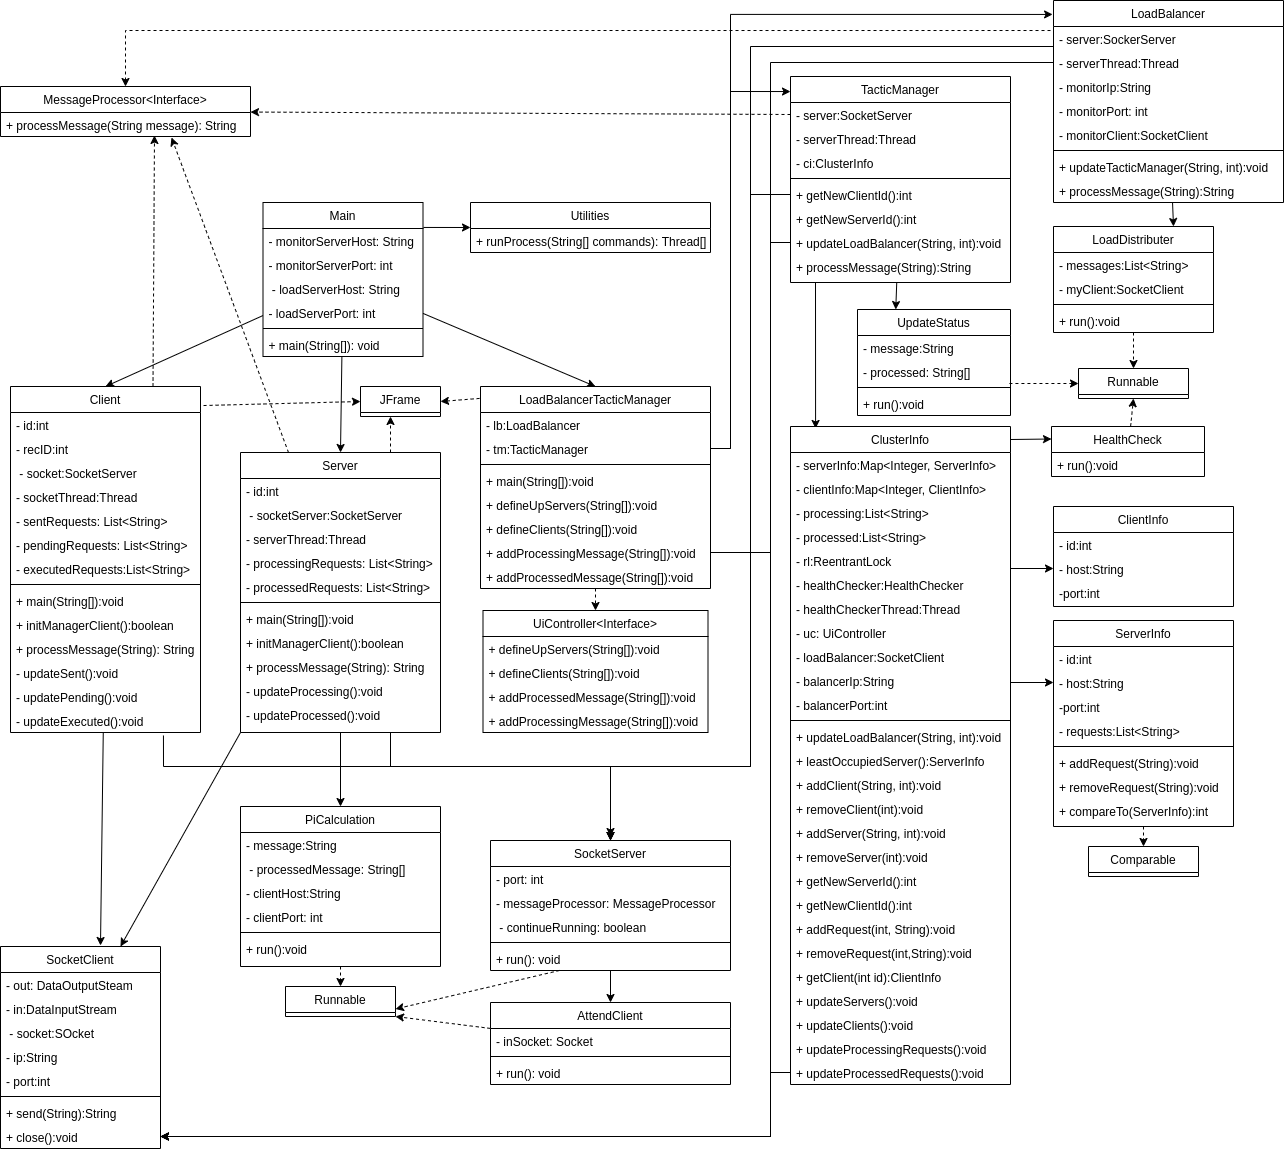
\includegraphics[width=\linewidth]{img/pa3Arch.png}
  \end{minipage}%
  \caption{Platform's architecture diagram.}
  \label{pa3Arch}
\end{figure} 

Then we have the SocketServer and SocketClient, which are wrapper classes for a WebSocket Server and a WebSocket Client.
They enabled us to use sockets personalized for our needs without worrying about the internal functioning of the original class, and in consequence keep our 
focus on our problem domain alone.
The only consideration we needed to make was that every entity that used the SocketServer needed to pass a MessageProcessor interface instance that would supply
all of the message processing logic.
The classes that implement MessageProcessor are the Client, the Server, the LoadBalancer and the TacticManager.
An internal class called AttendUser was added to our SocketServer to handle all the connections made to the WebSocket server in parallel.

\newpage
\subsection{User Interface} \label{ui} %%%%%%%%%%%%%%%%%%%%%%%%%% 

We defined from the very beginning that the GUIs would have to be as simple as possible, while providing both the basic and required elements for the user and 
additional features that would enrich their usability and empower the user.
The resulting interfaces are presented in this section.

...

\newpage
\section{Architecture Constraints} \label{constraints} %%%%%%%%%%%%%%%%%%%%%%%%%%%%%%%%%%%%%%%%%%%%%%%%%%%%%%%%%%%%%%%%%%%%%%%%%%%%%%%%%%%%%%%%%%%%%%%%%%%%%%%%%


\subsection{Quality Attributes Assurance} \label{qaa} %%%%%%%%%%%

\subsubsection{Performance}
% % 1. Replicas of computation: requests must be fairly distributed among the servers;
% % 2. Concurrency (must use ReentrantLock): each request runs on its own thread in a server;

\subsubsection{Availability}
% 1. Redundancy: to reallocate requests in case a server goes down;
% 2. Monitor: to supervise the cluster’s status (up/down servers (heartbeat), clients:
% identification, requests being processed, processed requests), etc., etc.). 

\subsubsection{Scalability}
% 1. Horizontal scalability: add new servers whenever necessary

\subsubsection{Usability}
% All GUI must be driven by Usability for the EVALUATION PROCESS: usage, trace, verification,
% validation, etc. You can resort to the tactics and anything else you think is necessary. The
% stakeholder will use the GUI to validate your implementation.

\subsection{Use Cases Compliance} \label{compliance} %%%%%%%%%%%


\newpage
\section{Additional Remarks} \label{remarks} %%%%%%%%%%%%%%%%%%%%%%%%%%%%%%%%%%%%%%%%%%%%%%%%%%%%%%%%%%%%%%%%%%%%%%%%%%%%%%%%%%%%%%%%%%%%%%%%%%%%%%%%%%%%%%%%%%%

\subsection{Documentation} \label{documentation} %%%%%%%%%%%%%%%%

Our attitude towards the developed code was to ensure it could be applied to other similar scenarios and reused in systems intended to be deployed in real scenarios.
With this in mind, we took great care with regards to code readability.
By maintaining a code style equal throughout the project and defining intuitive and self-explaining variable and method names, we made the code easy to understand
by someone already contextualized with Kafka.

Nevertheless, we wanted to make sure this was also true to someone looking at our project for the first time, so we resorted to the well-known Javadoc
\cite{javadoc} tool to manage all code documentation.
Comments were also added in key points throughout the code, including the scripts.

\subsection{Assignment Contributions} \label{contributions} %%%%%

As the entire development phase took place in a time where on-site cooperation was not possible, we resorted to online communication platforms to debate decisions
and discuss difficulties.
Team scheduling allowed us to work on the project simultaneously, so no member suffered from unbalanced workloads.
The dimension of the project did not appeal to the usage of repository pull requests and other synchronization tools.
However, each small solution was verified and agreed by both team members.

Having said this, it is difficult to isolate what each member actually implemented, as the influence of both is present in all components.
Nevertheless, one might say that each had stronger responsibilities on a set of project aspects:
Filipe took care of the execution of the individual Java processes and of the Shell scripts, while João developed the Kafka-related classes such as Consumer,
Producer and EntityAction; Filipe developed the Python script for generation of \texttt{CAR.TXT}, while João developed the Shell scripts for Kafka initialization
and deletion; each implemented 2 entities and each wrote a portion of this report; Filipe made sure everything was coherent throughout the report and the code
documentation, while João solved the most critical issues regarding the configuration of the topics.
In terms of work percentage, we believe it was about 50\% for each student.

\newpage
\section*{Conclusions} \label{conclusions} %%%%%%%%%%%%%%%%%%%%%%%%%%%%%%%%%%%%%%%%%%%%%%%%%%%%%%%%%%%%%%%%%%%%%%%%%%%%%%%%%%%%%%%%%%%%%%%%%%%%%%%%%%%%%%%%%%%%%

\begin{thebibliography}{9} %%%%%%%%%%%%%%%%%%%%%%%%%%%%%%%%%%%%%%%%%%%%%%%%%%%%%%%%%%%%%%%%%%%%%%%%%%%%%%%%%%%%%%%%%%%%%%%%%%%%%%%%%%%%%%%%%%%%%%%%%%%%%%%%%%%%%
  \bibliographystyle{Science}

  \bibitem{pisky}
  \textit{Pi in the sky: Calculating a record-breaking 31.4 trillion digits of Archimedes' constant on Google Cloud}.
  Taken from \href{https://web.archive.org/web/20191019023120/https://cloud.google.com/blog/products/compute/calculating-31-4-trillion-digits-of-archimedes-constant-on-google-cloud}{web.archive.org}.
  Retrieved May 2020.

  \bibitem{jorg}
  Arndt, Jorg \& Haenel, Christoph (2006).
  \textit{Pi Unleashed}, in Springer-Verlag.
  ISBN 978-3-540-66572-4.
  Retrieved May 2020.
  English translation by Catriona and David Lischka.

  % \bibitem{uml}
  %   Object Management Group,
  %   \textit{What is UML},
  %   \url{https://www.uml.org/what-is-uml.htm},
  %   accessed in March 2020.

\end{thebibliography}

\clearpage

\end{document}




















